\documentclass[a4paper,14pt]{extarticle}

% -------------------------------------
%                Пакеты
% -------------------------------------
\usepackage{geometry}
\geometry{a4paper,tmargin=2cm,bmargin=2cm,lmargin=3cm,rmargin=1cm}
\usepackage[T2A]{fontenc}
\usepackage[utf8]{inputenc}
\usepackage[english, main=russian]{babel}
\usepackage{textcomp}
\usepackage{indentfirst}
\usepackage{graphicx}
\graphicspath{{./images/}}
\usepackage{enumitem}
\usepackage{caption}
\usepackage{hyperref}
\hypersetup{unicode=true}

\DeclareCaptionLabelSeparator*{emdash}{~--- }
\captionsetup[figure]{labelsep=emdash,font=onehalfspacing,position=bottom}

\usepackage{tempora}
\usepackage{amsmath}
\usepackage{color}
\usepackage{listings}

\lstset{
  belowcaptionskip=1\baselineskip,
  breaklines=true,
  frame=L,
  xleftmargin=\parindent,
  language=C,
  showstringspaces=false,
  basicstyle=\footnotesize\ttfamily,
  keywordstyle=\bfseries\color{blue},
  commentstyle=\itshape\color{purple},
  identifierstyle=\color{black},
  stringstyle=\color{red},
  numbers=left,
  numberstyle=\tiny,
  stepnumber=1,
  numbersep=5pt
}

\linespread{1.3}
\sloppy
\clubpenalty=10000
\widowpenalty=10000

% -------------------------------------
%               Документ
% -------------------------------------
\begin{document}

% -------------------------------------
%           Титульный лист
% -------------------------------------
\begin{titlepage}
\thispagestyle{empty}

\vspace*{-60pt}
\begin{center}
  
\includegraphics[width=0.35\textwidth]{emblem}
\end{center}

\vspace{-25pt}
\hrule height2.3pt
\vspace*{-20.3pt}
\hrule

\vspace{4ex}
\begin{center}
  \small
  Министерство науки и высшего образования Российской Федерации\\
  Федеральное государственное бюджетное образовательное учреждение высшего образования\\
  «МГТУ им.~Н.\,Э.~Баумана (НИУ)»
\end{center}

\vspace{11em}
\begin{center}
  \Large\bfseries Летучка «Летучее видео»
\end{center}

\vspace{8em}
\begin{flushright}
  Студент группы ИУ9-21Б \textbf{Хромов М.\,А.}\\[2ex]
  Преподаватель \textbf{Посевин Д.\,П.}
\end{flushright}

\vfill
\begin{center}
  \textsl{Москва 2025}
\end{center}
\end{titlepage}

% -------------------------------------
\section{Сформулированное задание}
Из «Летучего видео» необходимо реализовать простую клиент--серверную
связку на сокетах TCP:
\begin{enumerate}[nosep]
  \item \textbf{Сервер} должен:
        \begin{itemize}[nosep]
          \item прослушивать порт \texttt{8080},
          \item принимать одно входящее соединение,
          \item вывести полученную строку в консоль и
          \item отослать подтверждение клиенту.
        \end{itemize}
  \item \textbf{Клиент} должен:
        \begin{itemize}[nosep]
          \item подключиться к локальному серверу по адресу
                \texttt{127.0.0.1:8080},
          \item отправить тестовую фразу
                «\texttt{Is There Anybody Out There?}»,
          \item получить ответ и вывести его.
        \end{itemize}
\end{enumerate}

% -------------------------------------
\section{Код программ}\label{sect:listings}

% ----------  Листинг 1 (client) ----------
\begin{figure}[!htb]
\begin{lstlisting}[caption={\texttt{tcp_client.c}},label={lst:client}]
#include <stdio.h>
#include <stdlib.h>
#include <string.h>
#include <sys/socket.h>
#include <arpa/inet.h>
#include <unistd.h>

#define PORT 8080
#define ADDR "127.0.0.1"

int main() {
    int client_fd;
    struct sockaddr_in peer;
    char buffer[1024] = {0};

    if ((client_fd = socket(AF_INET, SOCK_STREAM, 0)) < 0) {
        printf("Socket creation error\n");
        return 1;
    }

    peer.sin_family = AF_INET;
    peer.sin_port   = htons(PORT);
    if (inet_pton(AF_INET, ADDR, &peer.sin_addr) <= 0) {
        printf("Invalid address / not supported\n");
        return 1;
    }

    if (connect(client_fd, (struct sockaddr*)&peer, sizeof(peer)) < 0) {
        printf("Connection Failed\n");
        return 1;
    }

    char* msg = "Is There Anybody Out There?";
    send(client_fd, msg, strlen(msg), 0);
    printf("Message sent: %s\n", msg);

    read(client_fd, buffer, 1024);
    printf("Server response: %s\n", buffer);

    close(client_fd);
    return 0;
}
\end{lstlisting}
\end{figure}
\clearpage

% ----------  Листинг 2 (server) ----------
\begin{figure}[!htb]
\begin{lstlisting}[caption={\texttt{tcp_server.c}},label={lst:server}]
#include <stdio.h>
#include <stdlib.h>
#include <string.h>
#include <unistd.h>
#include <sys/socket.h>
#include <netinet/in.h>

#define PORT 8080
#define BUFFER_SIZE 1024

int main() {
    int server_fd, new_socket;
    struct sockaddr_in addr;
    int opt = 1, addrlen = sizeof(addr);
    char buffer[BUFFER_SIZE] = {0};

    if ((server_fd = socket(AF_INET, SOCK_STREAM, 0)) < 0) {
        perror("socket"); exit(EXIT_FAILURE);
    }
    if (setsockopt(server_fd, SOL_SOCKET, SO_REUSEADDR,
                   &opt, sizeof(opt))) {
        perror("setsockopt"); exit(EXIT_FAILURE);
    }

    addr.sin_family      = AF_INET;
    addr.sin_addr.s_addr = INADDR_ANY;
    addr.sin_port        = htons(PORT);

    if (bind(server_fd,(struct sockaddr*)&addr,sizeof(addr))<0){
        perror("bind"); exit(EXIT_FAILURE);
    }
    if (listen(server_fd,3) < 0) {
        perror("listen"); exit(EXIT_FAILURE);
    }
    printf("Server listening on %d...\n", PORT);

    if ((new_socket = accept(server_fd,(struct sockaddr*)&addr,
                             (socklen_t*)&addrlen)) < 0) {
        perror("accept"); exit(EXIT_FAILURE);
    }

    read(new_socket, buffer, BUFFER_SIZE);
    printf("Message received: %s\n", buffer);

    char* resp = "Message received by server";
    send(new_socket, resp, strlen(resp), 0);
    printf("Response sent\n");

    close(new_socket);
    close(server_fd);
    return 0;
}
\end{lstlisting}
\end{figure}
\clearpage

% -------------------------------------
\section{Скриншот результата}
\begin{center}
  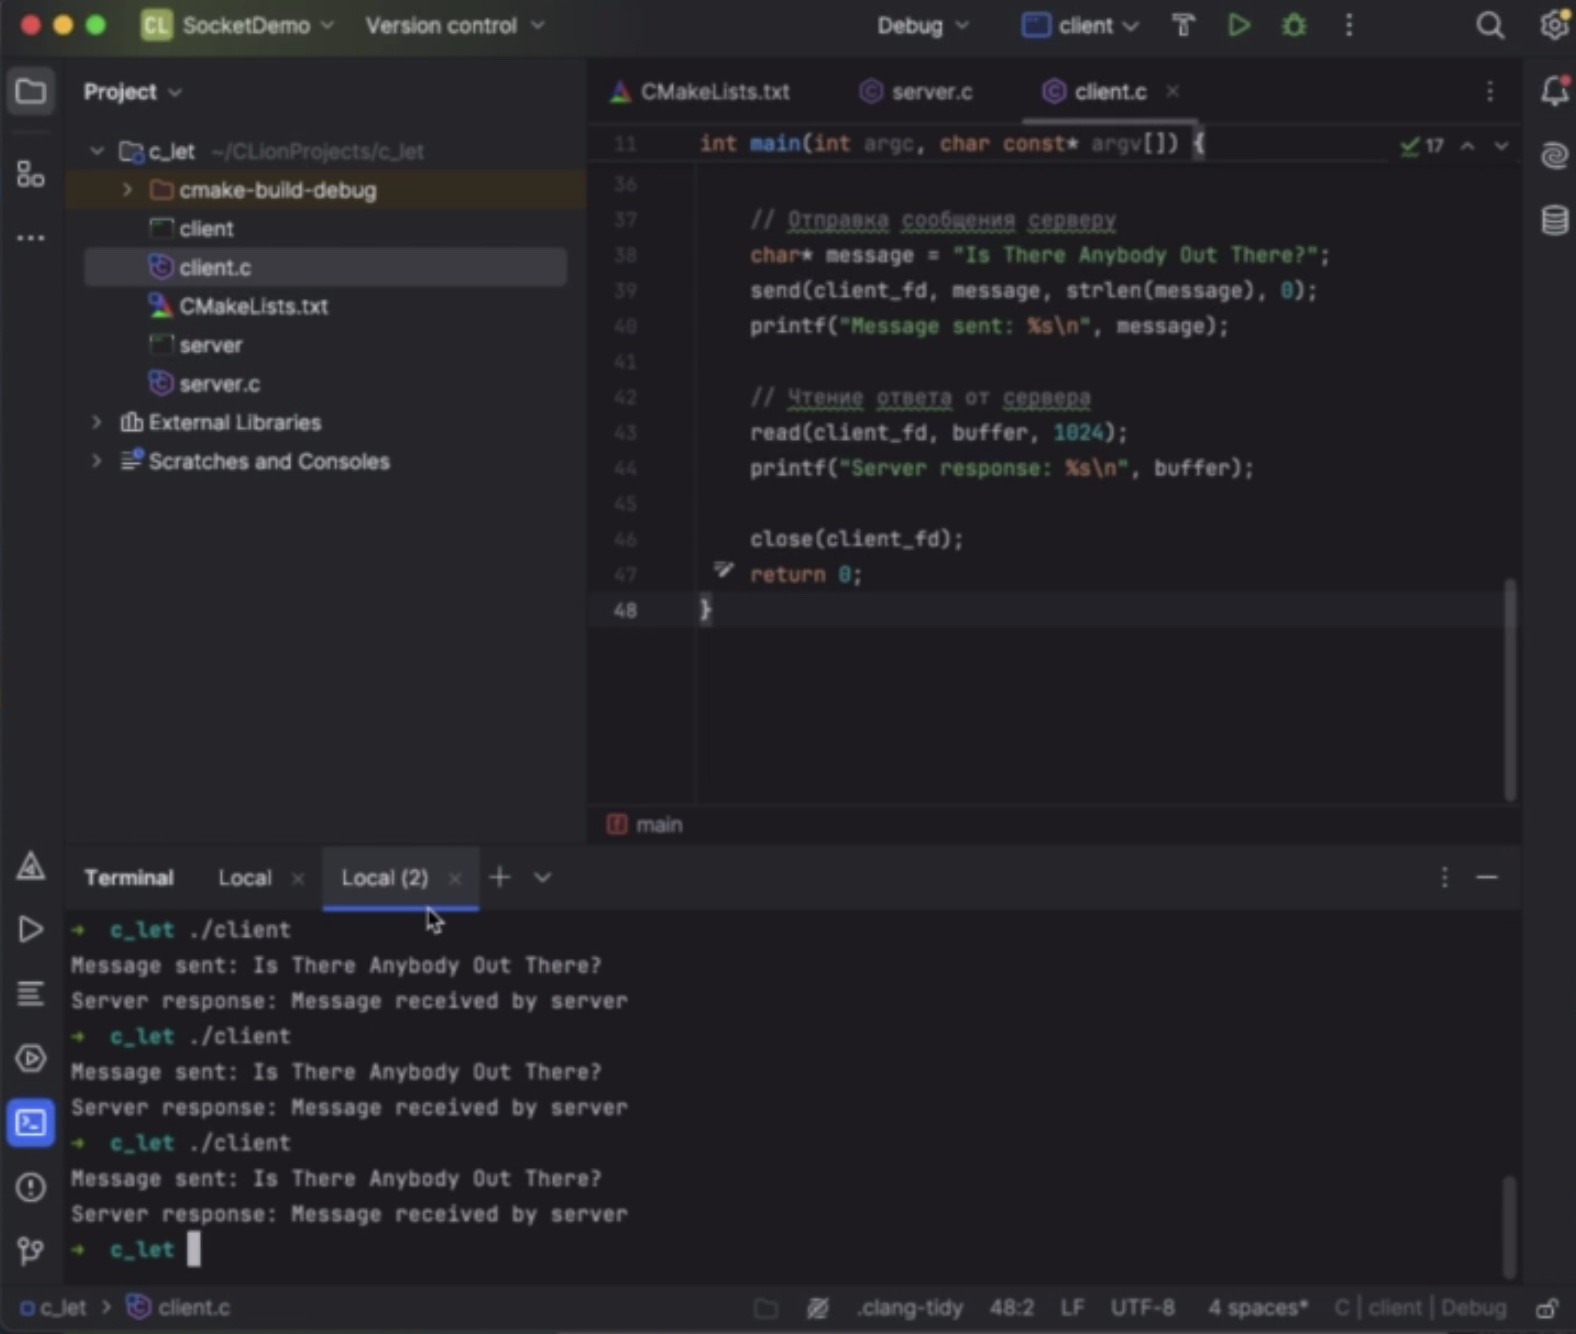
\includegraphics[width=0.8\textwidth]{фото30.jpeg}
  \captionof{figure}{Тестовый запуск: обмен сообщениями между клиентом и сервером}
\end{center}

% -------------------------------------
\section{Вывод}
Выполнено задание из Летучего видео
\end{document}
